\chapter{Optimisation}
\section{Motivation}
\begin{quote}
    \textit{"Users expect miracles! \dots Data management systems can actually accommodate some \dots - Holger Pirk"}
\end{quote}
\begin{itemize}
    \item Users want zero-overhead, the system should be as fast as hand-written \& optimised code.
    \item The database is expected to learn from data (e.g second run of a query is faster)
    \item System must be highly flexible (users can create relations, indices, build complex queries without needing to upgrade/reconfigure/recompile any part of the DBMS)
\end{itemize}
In reality current \textit{DBMS} generally succeed in meeting these \textit{miraculous} expectations.

\subsection{Query Optimisers vs Optimising Compilers}
A query optimiser is similar to a compiler's optimiser:
\begin{itemize}
    \item Representation of code is transformed through several representations, some logical (e.g AST, three address code), some physical (e.g x86 specific IR, assembly representation)
    \item Correctness under optimisations (\textbf{primary objective}), performance of optimiser queries (\textbf{secondary objective}).
    \item Limitations on time to optimise (i.e developers don't want to wait excessively long to compile simple programs)
\end{itemize}
The main difference is timing of access to code and input data.
\begin{center}
    \begin{tabular}{l l l}
                                    & \textbf{Code/Query} & \textbf{Input Data} \\
        \textbf{Compiler Optimiser} & At compile time     & Unknown             \\
        \textbf{Query Optimiser}    & At query time       & Known before query  \\
    \end{tabular}
\end{center}

\begin{sidenotebox}{Profile Guided Optimisation}
    A compiler optimiser (at compile) does not have access to the input data (at runtime). However this is not entirely \textit{technically} true. We can compile an instrumented version of the code, run with some representative input data, profile and provide this feedback to the compiler to guide optimisation.
    \begin{minted}{bash}
g++ -fprofile-generate myprog.cpp # Compile instrumented version
./myprog.cpp                      # Generates myprog.gcda
g++ -fprofile-use myprog.cpp      # Use profile when optimising
    \end{minted}
\end{sidenotebox}

Correctness is difficult.
\begin{itemize}
    \item ANSI SQL semantics are not formally defined (though some have been \href{https://dl.acm.org/doi/10.1145/111197.111212}{developed}).
    \item Need to test against complex queries, numerous edge cases, with many combinations of optimisations (much the same as with compiler's optimisers).
\end{itemize}

\begin{sidenotebox}{Fuzzing}
    One common practice for testing compilers (and DBMS) is to randomly generate potential queries, and then test for differences in results from optimised and un-optimised.
    \begin{center}
        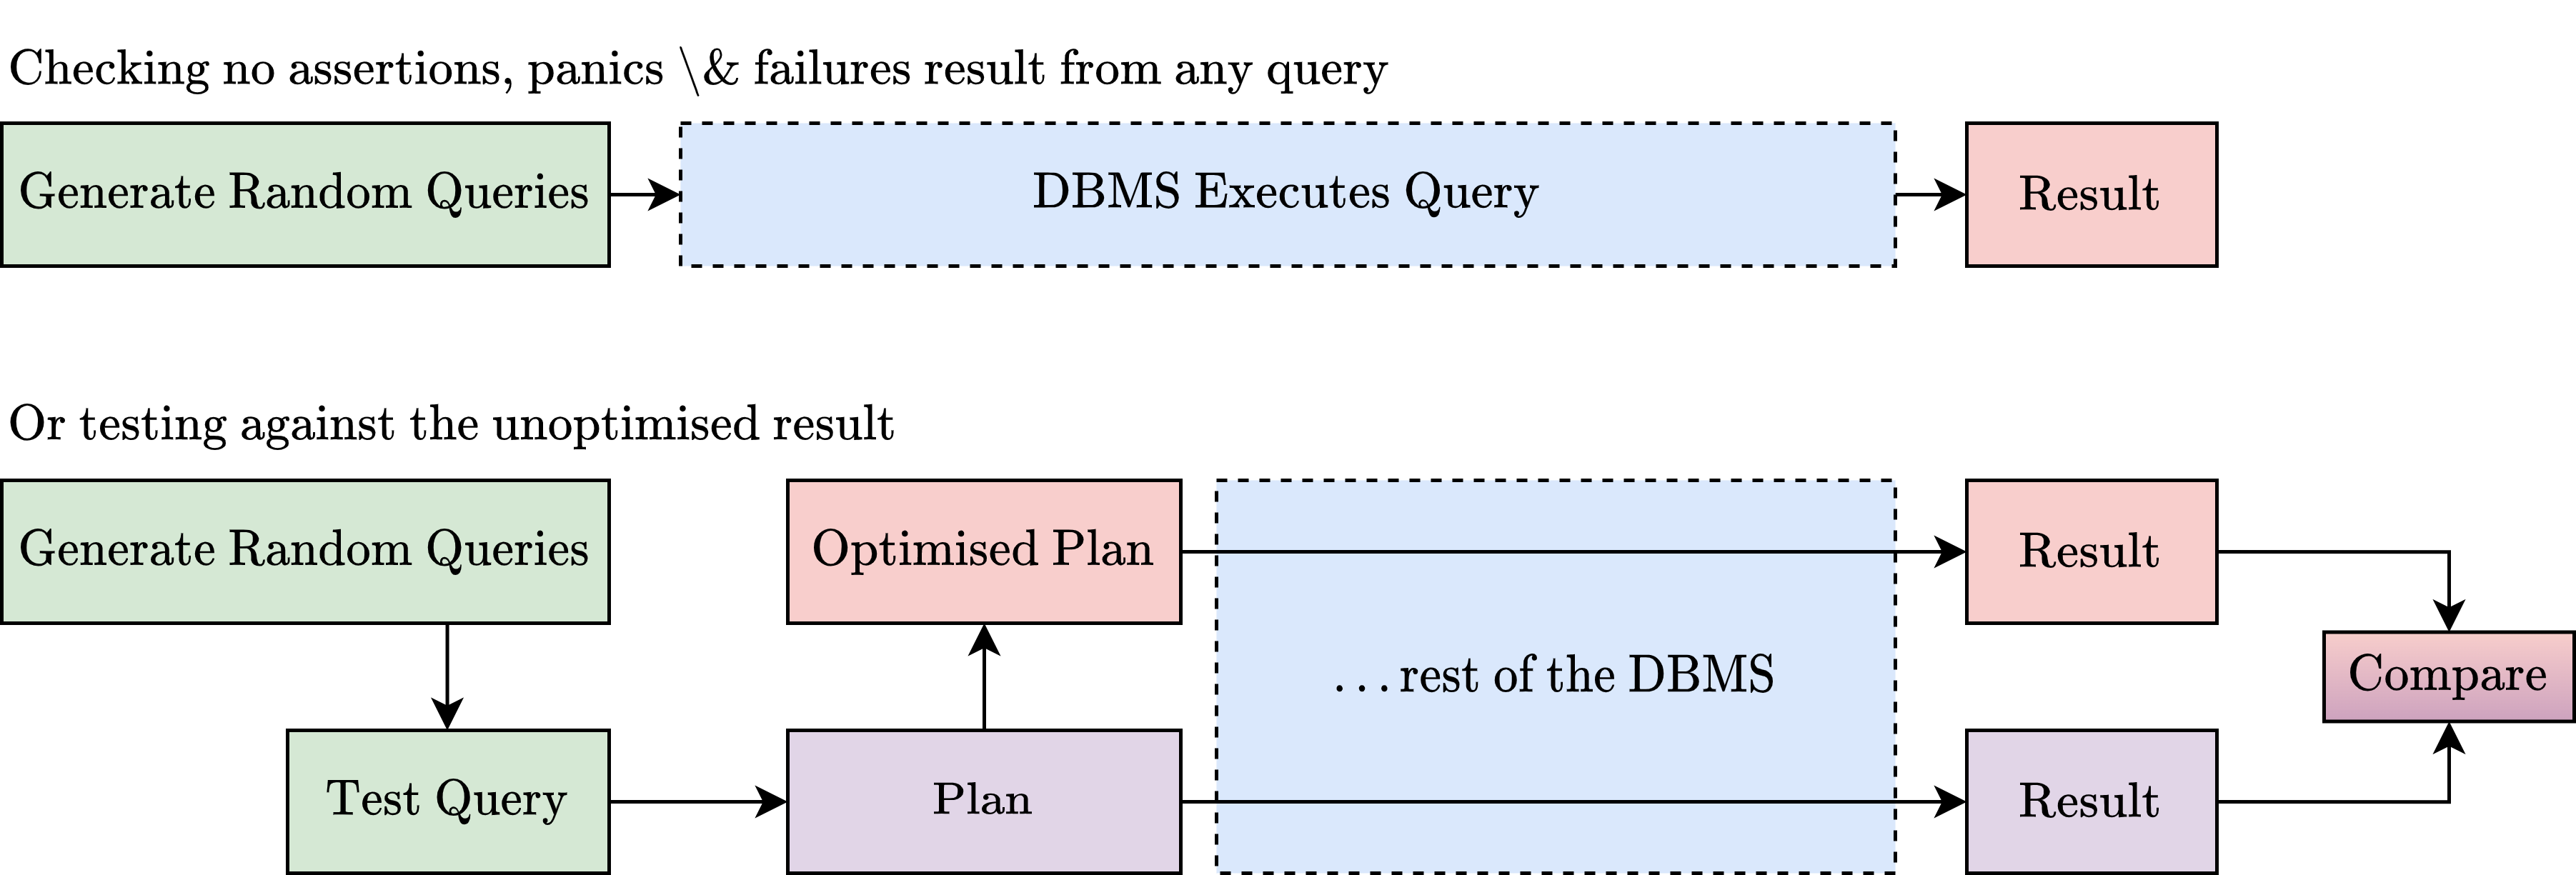
\includegraphics[width=.8\textwidth]{optimisation/images/fuzzing.drawio.png}
    \end{center}
    For example \href{https://github.com/anse1/sqlsmith}{SQLsmith} can be used to generate random SQL queries, and has been used to test and find bugs in Postgres, sqlite3, monetdb and more (see the \href{https://github.com/anse1/sqlsmith/wiki#score-list}{score list}).
\end{sidenotebox}

\subsection{Query Equivalence}
\begin{definitionbox}{Semantic Equivalence}
    Plans are \textit{semantically equivalent} if they provable produce the same output on any dataset.
\end{definitionbox}
\begin{definitionbox}{Closure (Mathematics)}
    (\textit{Simplified}) A set is closed under an operation if the operation produces elements of the same set.
    \begin{itemize}
        \item $\mathbb{N}$ is closed under $+$, but not under $-$ (can produce negative numbers)
        \item \textit{Relational algebra} is closed (the set of possible relations is closed under the operators of the algebra).
    \end{itemize}
\end{definitionbox}
\begin{center}
    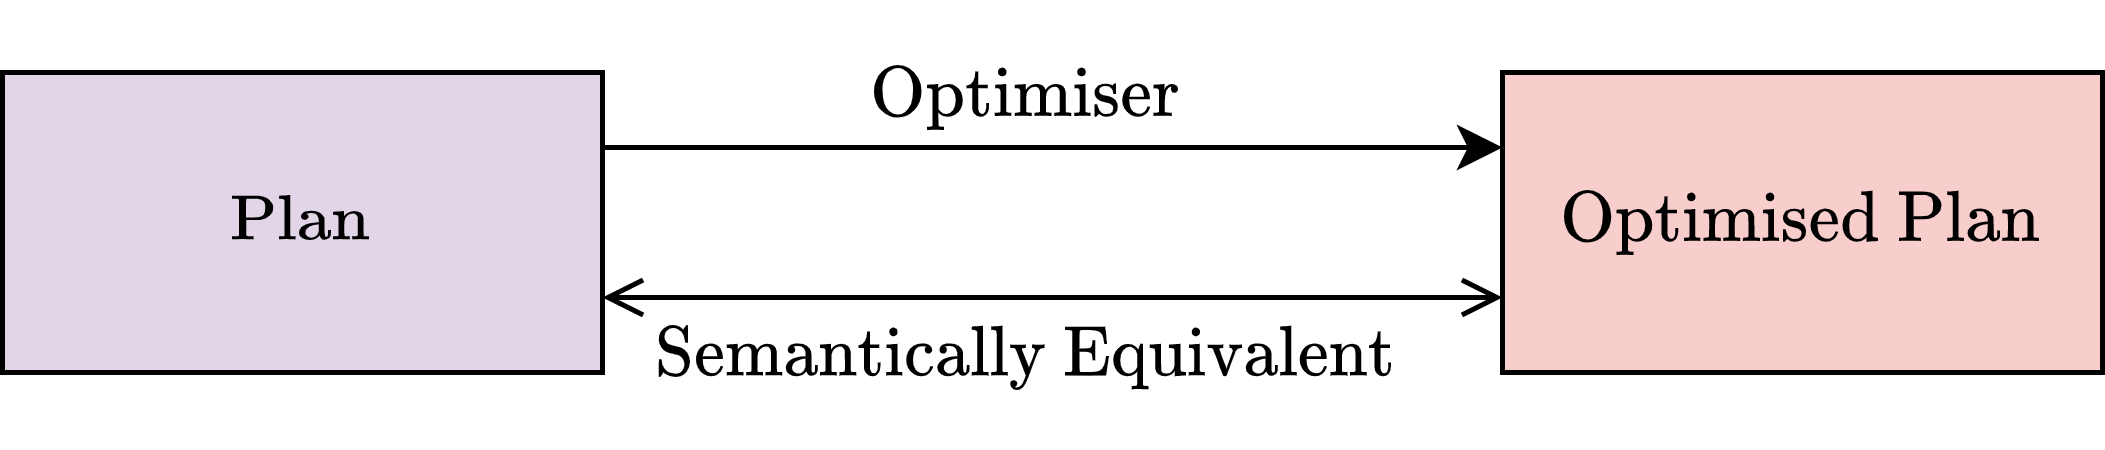
\includegraphics[width=.7\textwidth]{optimisation/images/semantic_equivalence.drawio.png}
\end{center}
As \textit{relational algebra} is closed, operators are easily composable.
\begin{itemize}
    \item We can determine equivalences between compositions of operators.
    \item Substitutions of a part of a plan with an equivalent, results in a new equivalent plan.
    \item We can use this to transform plans into more optimal (but equivalent) plans.
\end{itemize}

\begin{sidenotebox}{MonetDB Optimiser}
    MonetDB is an open source, in-memory, decomposed database. Its \href{https://github.com/MonetDB/MonetDB/blob/master/monetdb5/optimizer/optimizer.c}{optimiser} includes implementations for the optimisations discussed in this chapter (e.g \href{https://github.com/MonetDB/MonetDB/blob/master/monetdb5/optimizer/opt_pushselect.c}{selection pushdown})
\end{sidenotebox}

\section{Peephole Transformations}
\begin{quote}
    \textit{"An equivalent transformation of a subplan is an equivalent transformation of the entire plan."}
\end{quote}
A set of rules for transforming small subplans (peephole) is applied while traversing the plan.

\begin{sidenotebox}{WACC Peephole}
    This is the same idea as peephole optimisations discussed in the WACC project and 50006 - Compilers.
    \begin{minipage}{.49\textwidth}
        \begin{minted}{asm}
mov r1, r1 ; redundant move
        
        \end{minted}
    \end{minipage} \hfill \begin{minipage}{.49\textwidth}
        \begin{minted}{asm}
str r4, [sp, #8] ; overwritten store 
str l3, [sp, #8]
        \end{minted}
    \end{minipage}
\end{sidenotebox}

\begin{itemize}
    \item Need some order with which to traverse the plan
    \item Need a set of patterns/rules to apply.
\end{itemize}

\subsection{Avoiding Cycles}
\begin{definitionbox}{Analytically Optimal Plan}
    The final plan output of the optimiser (not necessarily the most optimal plan).
\end{definitionbox}
\begin{center}
    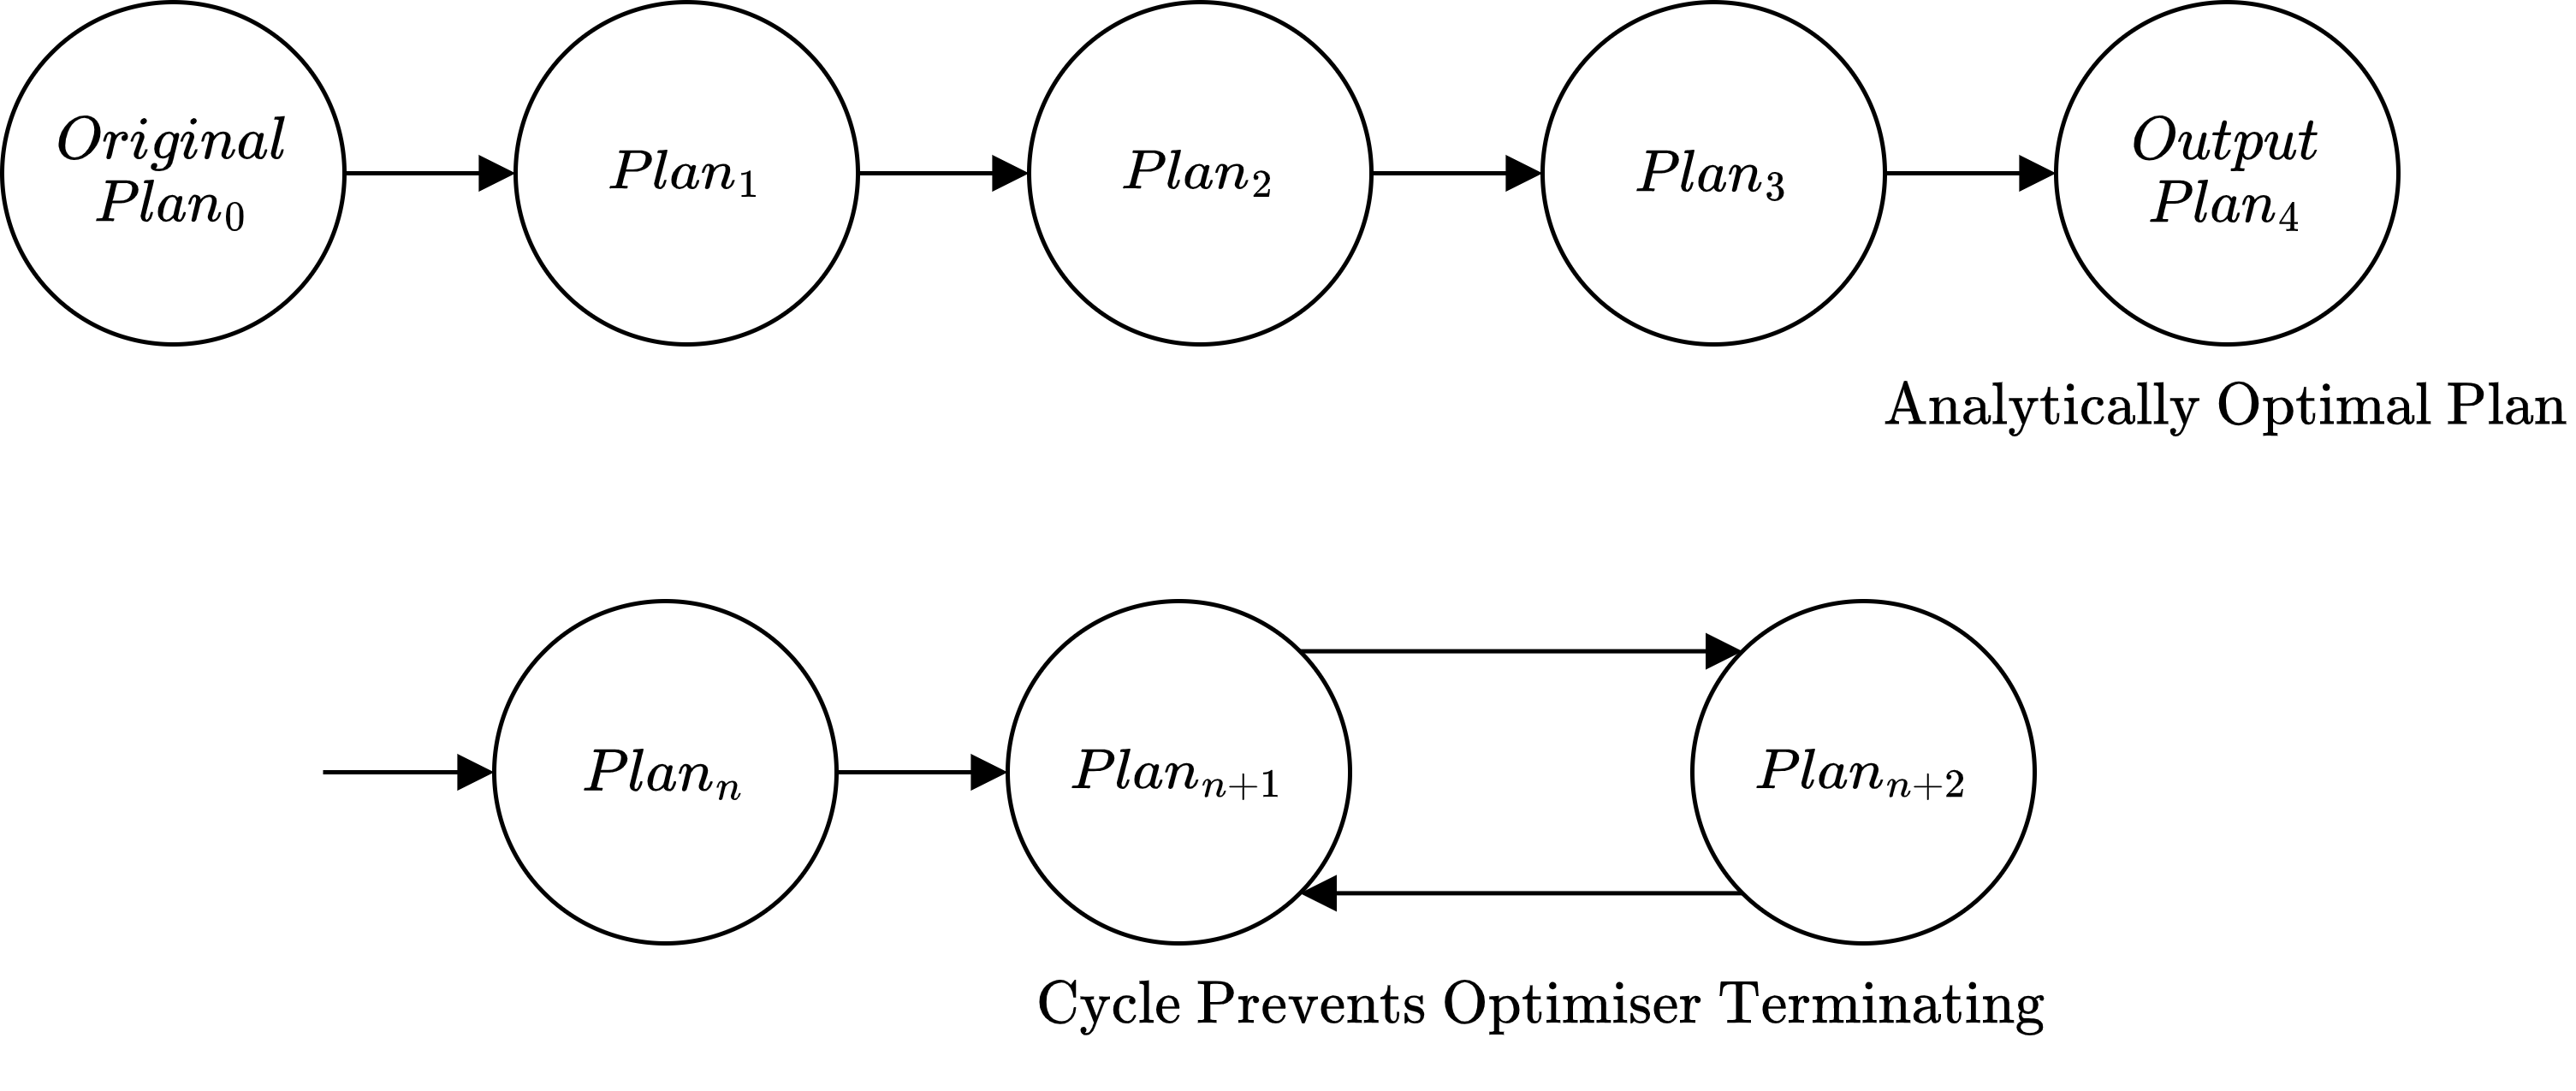
\includegraphics[width=.8\textwidth]{optimisation/images/optimiser_cycle.drawio.png}
\end{center}
Avoiding this requires careful rule selection.

\subsection{Branches}
\begin{center}
    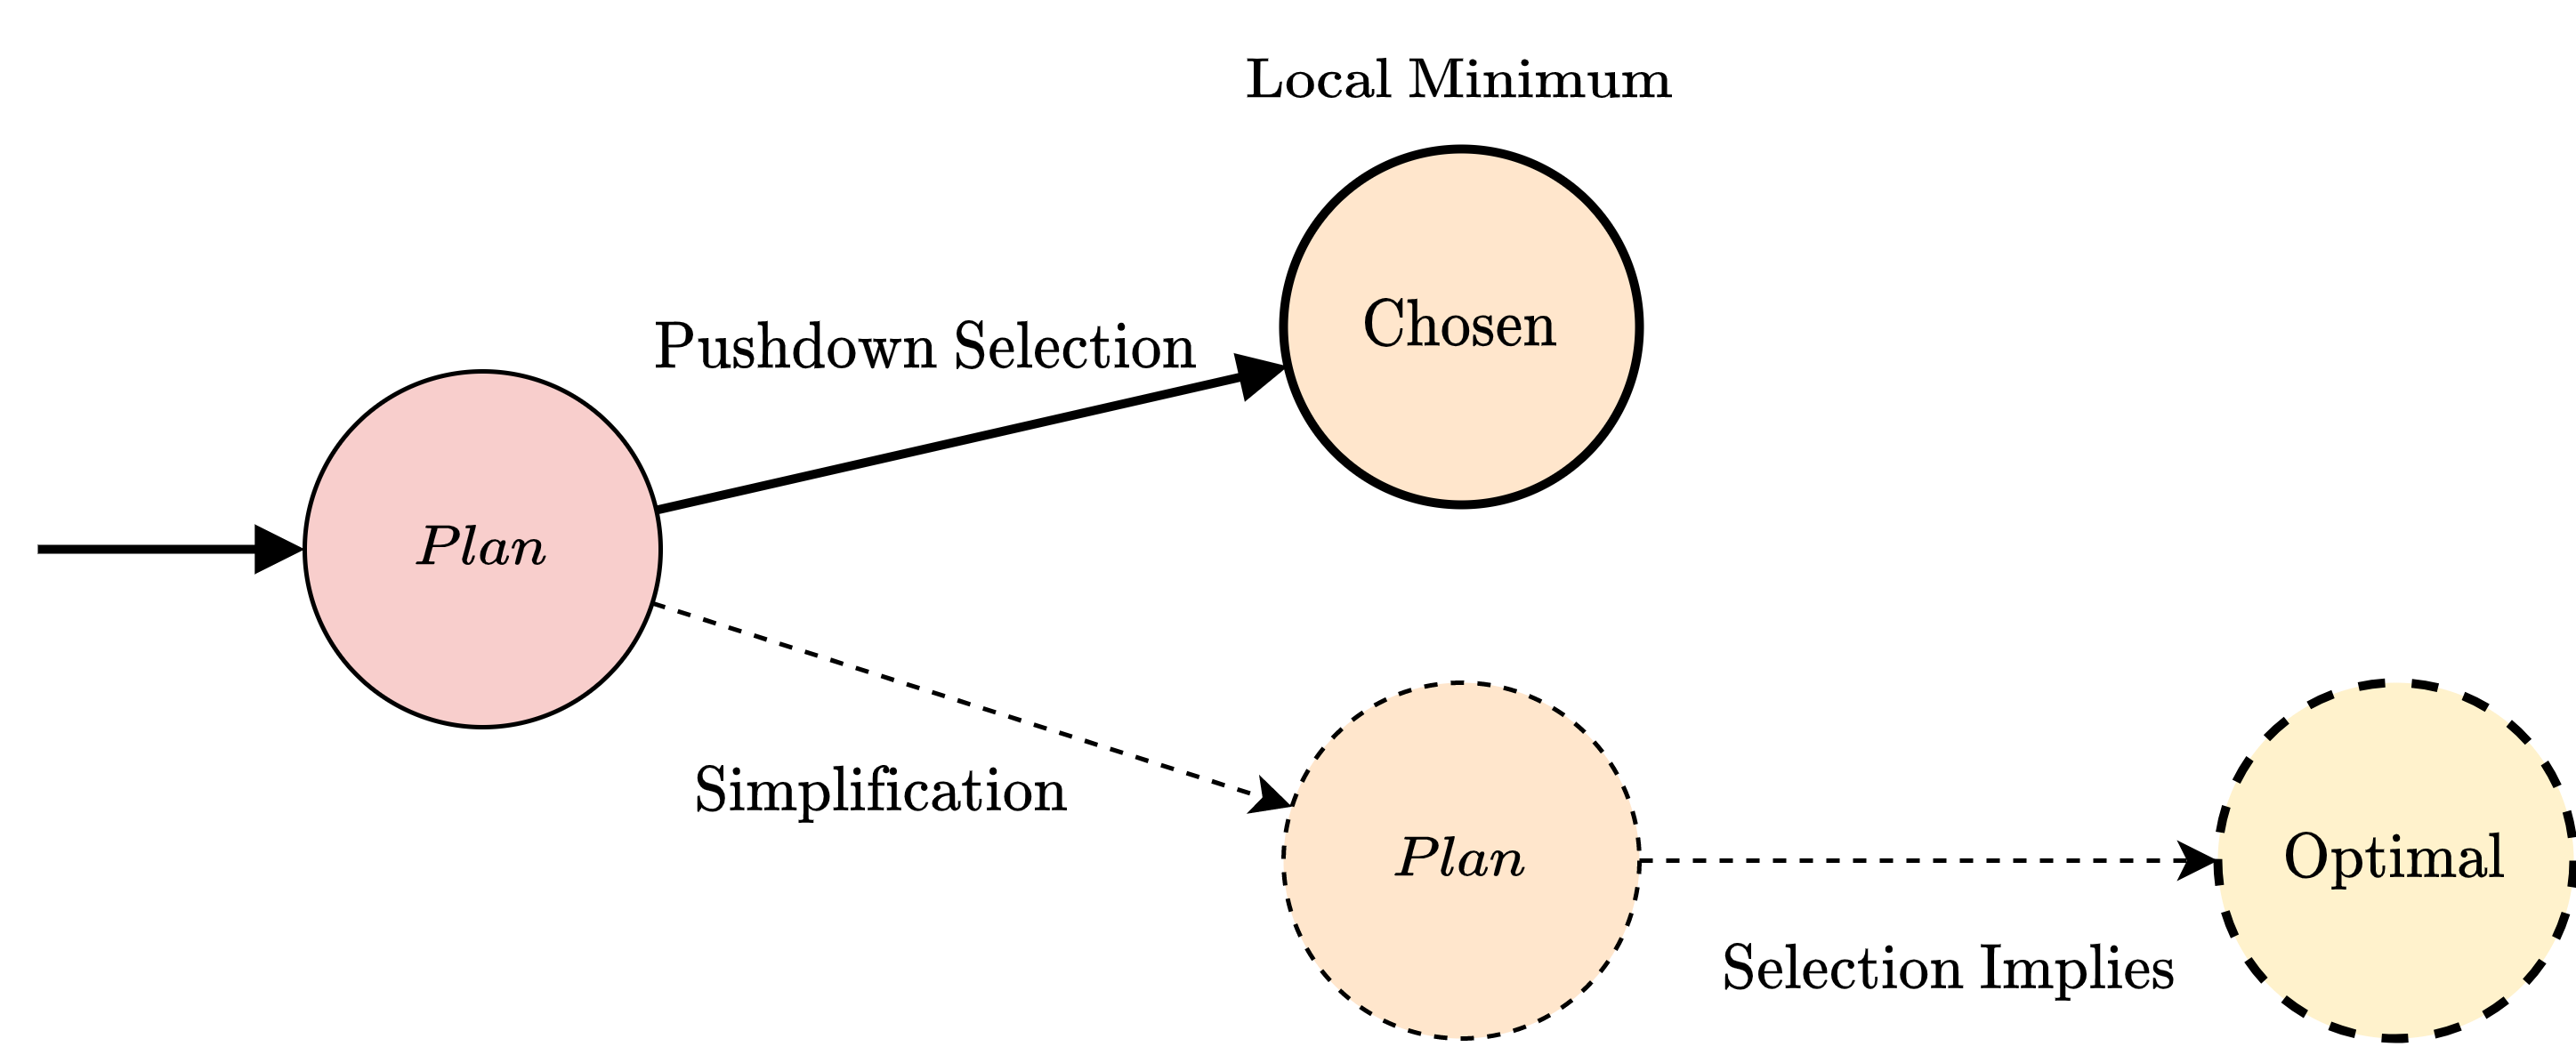
\includegraphics[width=.8\textwidth]{optimisation/images/optimiser_branch.drawio.png}
\end{center}
As many possible rules may be applied, some strategy is needed to determine which to apply (e.g just order the rules).

\begin{tabbox}{prosbox}
    \textbf{Simplicity} & Very easy to implement (particularly with pattern matching). \\
    \textbf{Time} & Matching and applying rules is faster than more holistic approaches. \\
    \textbf{Verifiability} & Can check each rule for correctness by checking if all rules produce semantically equivalent sub-plans. \\
    \textbf{Composability} & Can easily add new rules to be composed with previous, rules can enable new rules to be applied. \\
\end{tabbox}
\begin{tabbox}{consbox}
    \textbf{Loops} & Developer must be careful to not introduce potential loops in rule application. \\
    \textbf{Local Optima} & Typically many choices of rule to apply $\Rightarrow$ local optima. \\
\end{tabbox}

\section{Classifying Optimisation}
\begin{center}
    \begin{tabular}{l p{.8\textwidth}}
        \textbf{Algorithm} & The implementation of operators (e.g joins).                        \\
        \textbf{Data}      & Data \& metadata held by the system (e.g cardinalities, histograms) \\
    \end{tabular}
\end{center}

\begin{center}
    \begin{tabular}{l l l c c}
                                       &          &                     & \multicolumn{2}{c}{\textbf{Algorithm}}                     \\
                                       &          &                     & Agnostic                               & Aware             \\
                                       &          &                     & \textit{Logical}                       & \textit{Physical} \\
        \multirow{2}{*}{\textbf{Data}} & Agnostic & \textit{Rule-Based} & $\bullet$                              & $\bullet$         \\
                                       & Aware    & \textit{Cost-Based} & $\bullet$                              & $\bullet$         \\
    \end{tabular}
\end{center}
In DBMS optimisations are defined as operating on \textit{logical} or \textit{physical plans}, and are either \textit{rule-based} or \textit{cost-based}.
\begin{center}
    \begin{tabular}{l l p{.7\textwidth}}
        \textbf{Logical}    & \textit{Algorithm-Agnostic} & Deals only with relational algebra.                                                                                                                                   \\
        \textbf{Physical}   & \textit{Algorithm-Aware}    & Can use different operator implementations, indices etc.                                                                                                              \\
        \textbf{Rule-Based} & \textit{Data-Agnostic}      & Applying optimisation rules that are almost always beneficial.                                                                                                        \\
        \textbf{Cost-Based} & \textit{Data-Aware}         & Using data to estimate the cost of operations in order to determine which transformations to apply (e.g reordering selections based on each's estimated selectivity). \\
    \end{tabular}
\end{center}

% plan cycles
% diverging plans

\section{Logical Optimisation}
In order to demonstrate logical optimisation we use a representation of
(pseudo) relational algebra in Haskell.
\begin{center}
    \begin{minipage}{.5\textwidth}
        \begin{minted}{haskell}
    data Operator = 
      Scan Table
    | Select      Operator Predicate
    | Project     Operator RowTrans
    | Product     Operator Operator
    | Join        Operator Operator Predicate
    | Difference  Operator Operator
    | Union       Operator Operator
    | Aggregation Operator AggFun
    | TopN        Operator SortBy
    \end{minted}
    \end{minipage} \hfill \begin{minipage}{.49\textwidth}
        \begin{itemize}
            \item Purely logical representation, Processing model \& operator implementations not specified.
            \item Other functions for predicting cost, ordering predicates defined
            \item Using \mintinline{haskell}{data} to allow for easy pattern matching, rather than using an operator typeclass.
        \end{itemize}
    \end{minipage}
\end{center}
We include basic functions for applying transformations to the plan:
\begin{minted}{haskell}
-- Apply some transformation to all children of an operator
apply :: (Operator -> Operator) -> Operator -> Operator

-- Maybe peephole optimise operator (do not traverse to children)
type Peephole = Operator -> Maybe Operator

-- Optimise a plan 
type Optimiser = Operator -> Operator
\end{minted}
hence we can create functions to take a set of \textit{rules} and some \textit{traversal} and create an optimiser we can apply to plans. For example:
\begin{minted}{haskell}
-- Continue traversing until making an optimisation, then return to root.
-- As optimisations on either side of a join, difference, or union are 
-- independent, traverse both independently (with apply).
root :: Peephole -> Optimiser
root peep orig 
  = case peep orig of
    Just opt -> opt
    Nothing  -> apply (root peep) orig
\end{minted}
All that remains is to determine the \mintinline{haskell}{Peephole}'s rules.
\begin{sidenotebox}{Your turn!}
    One way to further simplify the representation is to embed RA as a DSL within another language. \href{https://racket-lang.org/}{Racket} (\textit{the language oriented programming language}) is designed for this. Have a go with your own implementation!
\end{sidenotebox}
\subsection{Rule Based Logical Optimisation}
The optimiser has a set of (almost) universally beneficial rules applied to transform the plan.
\\
\\ Some basic assumptions from which to derive rules include:
\begin{itemize}
    \item Higher cardinality (more tuples) $\Rightarrow$ Higher Cost
    \item Joins usually increase cardinality, or leave unchanged
    \item Selections reduce cardinality
    \item Aggregations reduce cardinality
    \item Data access is more expensive than function evaluation (can assume generally, without exposing operator implementation)
\end{itemize}

\begin{tabbox}{prosbox}
    \textbf{Portable} & Implementation independent (i.e can change processing model without needing to change optimisations - reduced developer maintenance requirements). \\
    \textbf{Robust} & Small changes in the data or algorithm do not dramatically change performance \\
\end{tabbox}
\begin{tabbox}{consbox}
    \textbf{Wrong} & The transformations need to be almost always beneficial, so must be conservative with choosing rules. A wrong rule can significantly reduce performance. \\
    \textbf{Brittle} & A rule removal/addition can result in significant performance changes. \\
    \textbf{Unprincipled} & Rules tend to be ad-hoc or arbitrary, they are backed by assumptions - not information about workload. \\
    \textbf{Loops} & As with \textit{peephole} in general. \\
\end{tabbox}

\begin{minted}{haskell}
-- creating peephole opt for logical rule-based optimisation
logicalRuleBased :: Peephole

-- at the end is a catch-all base case
logicalRuleBased _ = Nothing
\end{minted}

\subsubsection{Selection Pushdown}
\begin{center}
    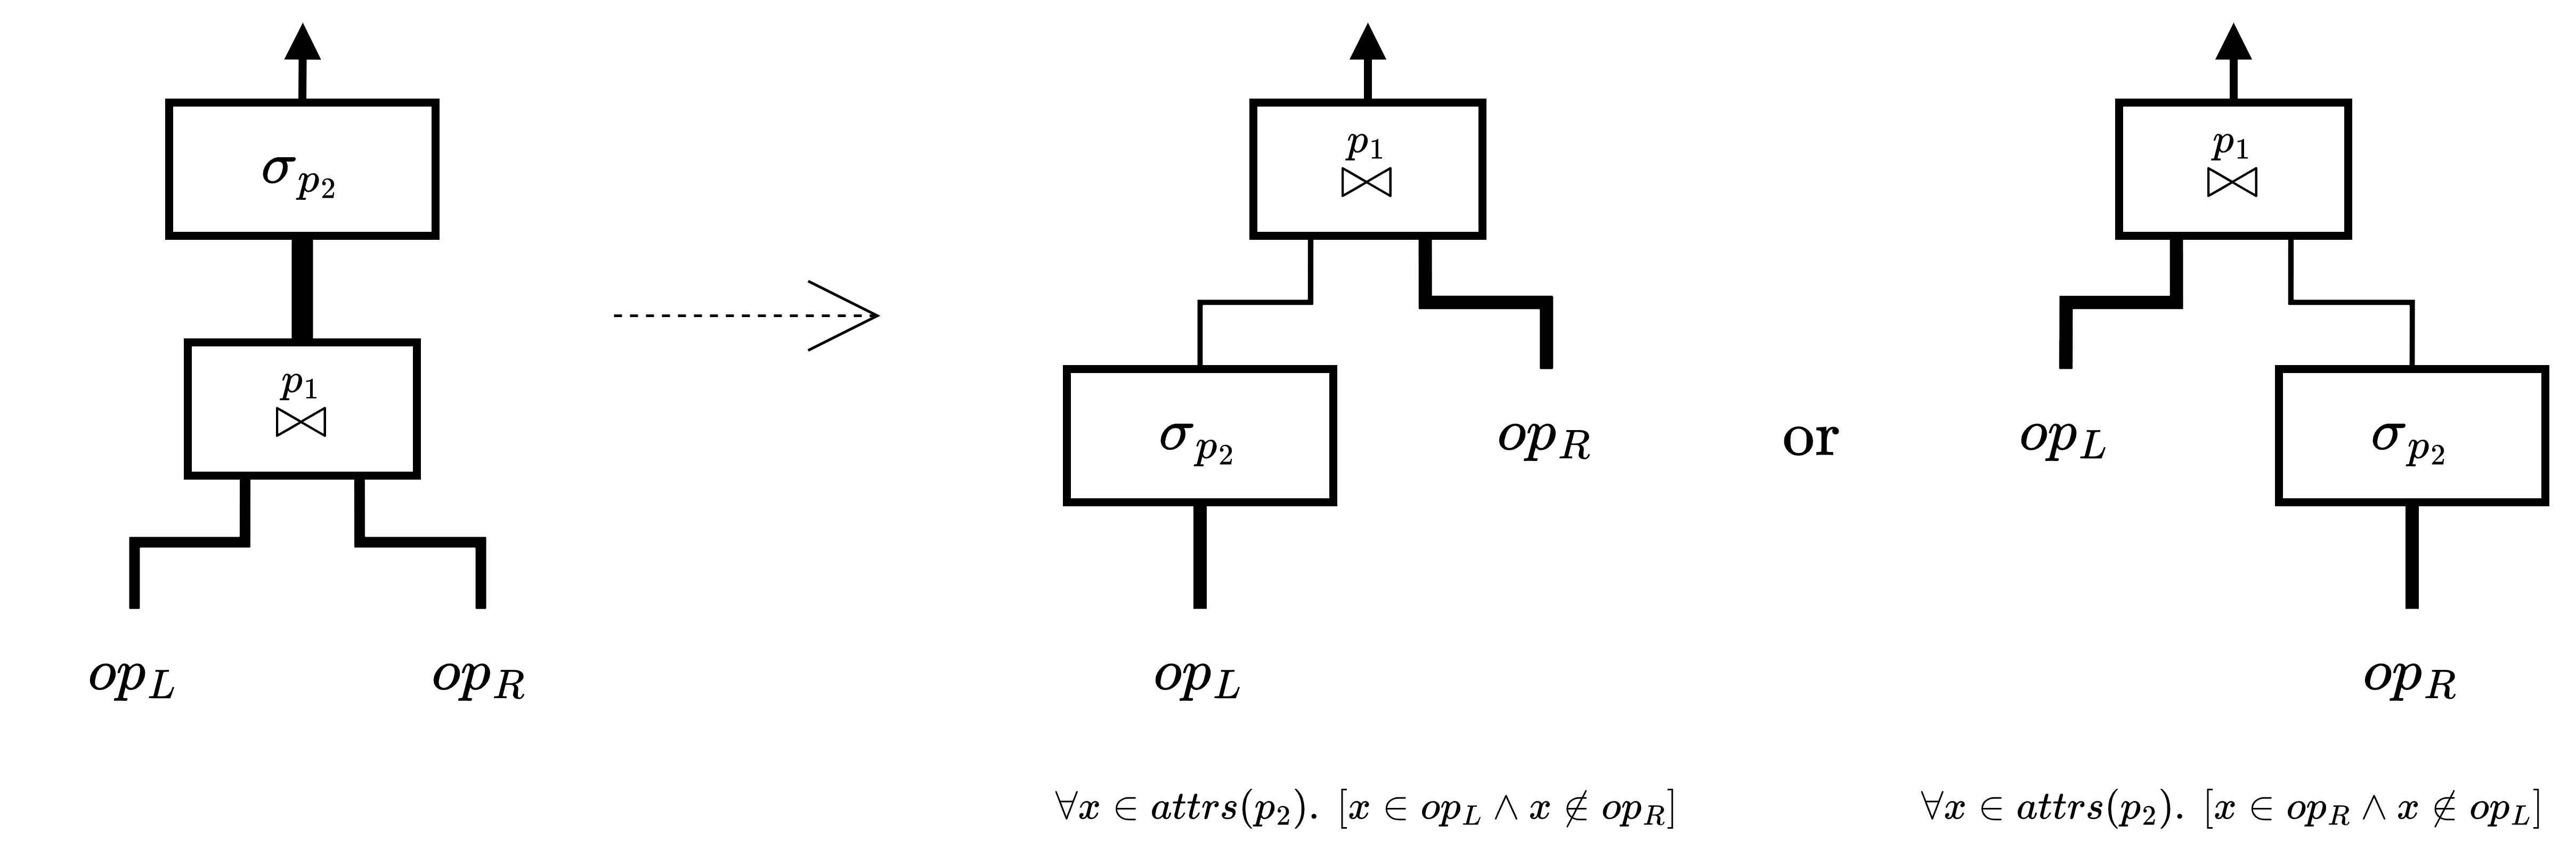
\includegraphics[width=.9\textwidth]{optimisation/images/push_down_selection.drawio.png}
\end{center}
Selections can be \textit{pushed down} through joins if they only use attributed from one side of the join.
\begin{itemize}
    \item As selections are pipelineable, this often a good optimisation when the underlying processing model is volcano.
\end{itemize}
\begin{minted}{sql}
SELECT * FROM opL JOIN opR WHERE p2;
\end{minted}
\dots is optimised to \dots
\begin{minted}{sql}
SELECT * FROM (SELECT * FROM opL WHERE p2) JOIN opR;
-- or
SELECT * FROM opL JOIN (SELECT * FROM opR WHERE p2);
\end{minted}
\begin{minted}{haskell}
-- assuming attributes names of opR and opL different
logicalRuleBased (Select (Join opL opR p1) p2) 
  | attributes opR `containsAll` selectCols p2 = Just (Join opL (Select opR p2 s2) p1 s1)
  | attributes opL `containsAll` selectCols p2 = Just (Join (Select opL p2 s2) opR p1 s1)
\end{minted}

\begin{examplebox}{Dont push me down!}
    Is \textit{selection pushdown} ever not very beneficial, provide some edge cases?
    \tcblower
    \begin{itemize}
        \item If the selectivity of the selection is $100\%$ and the join does not increase cardinality (no benefit).
        \item If the join significantly reduces cardinality.
    \end{itemize}
    \unfinished
    % Lecture mentions function calls vs access & fk index based joins
\end{examplebox}

\subsubsection{Selection Ordering}
\begin{center}
    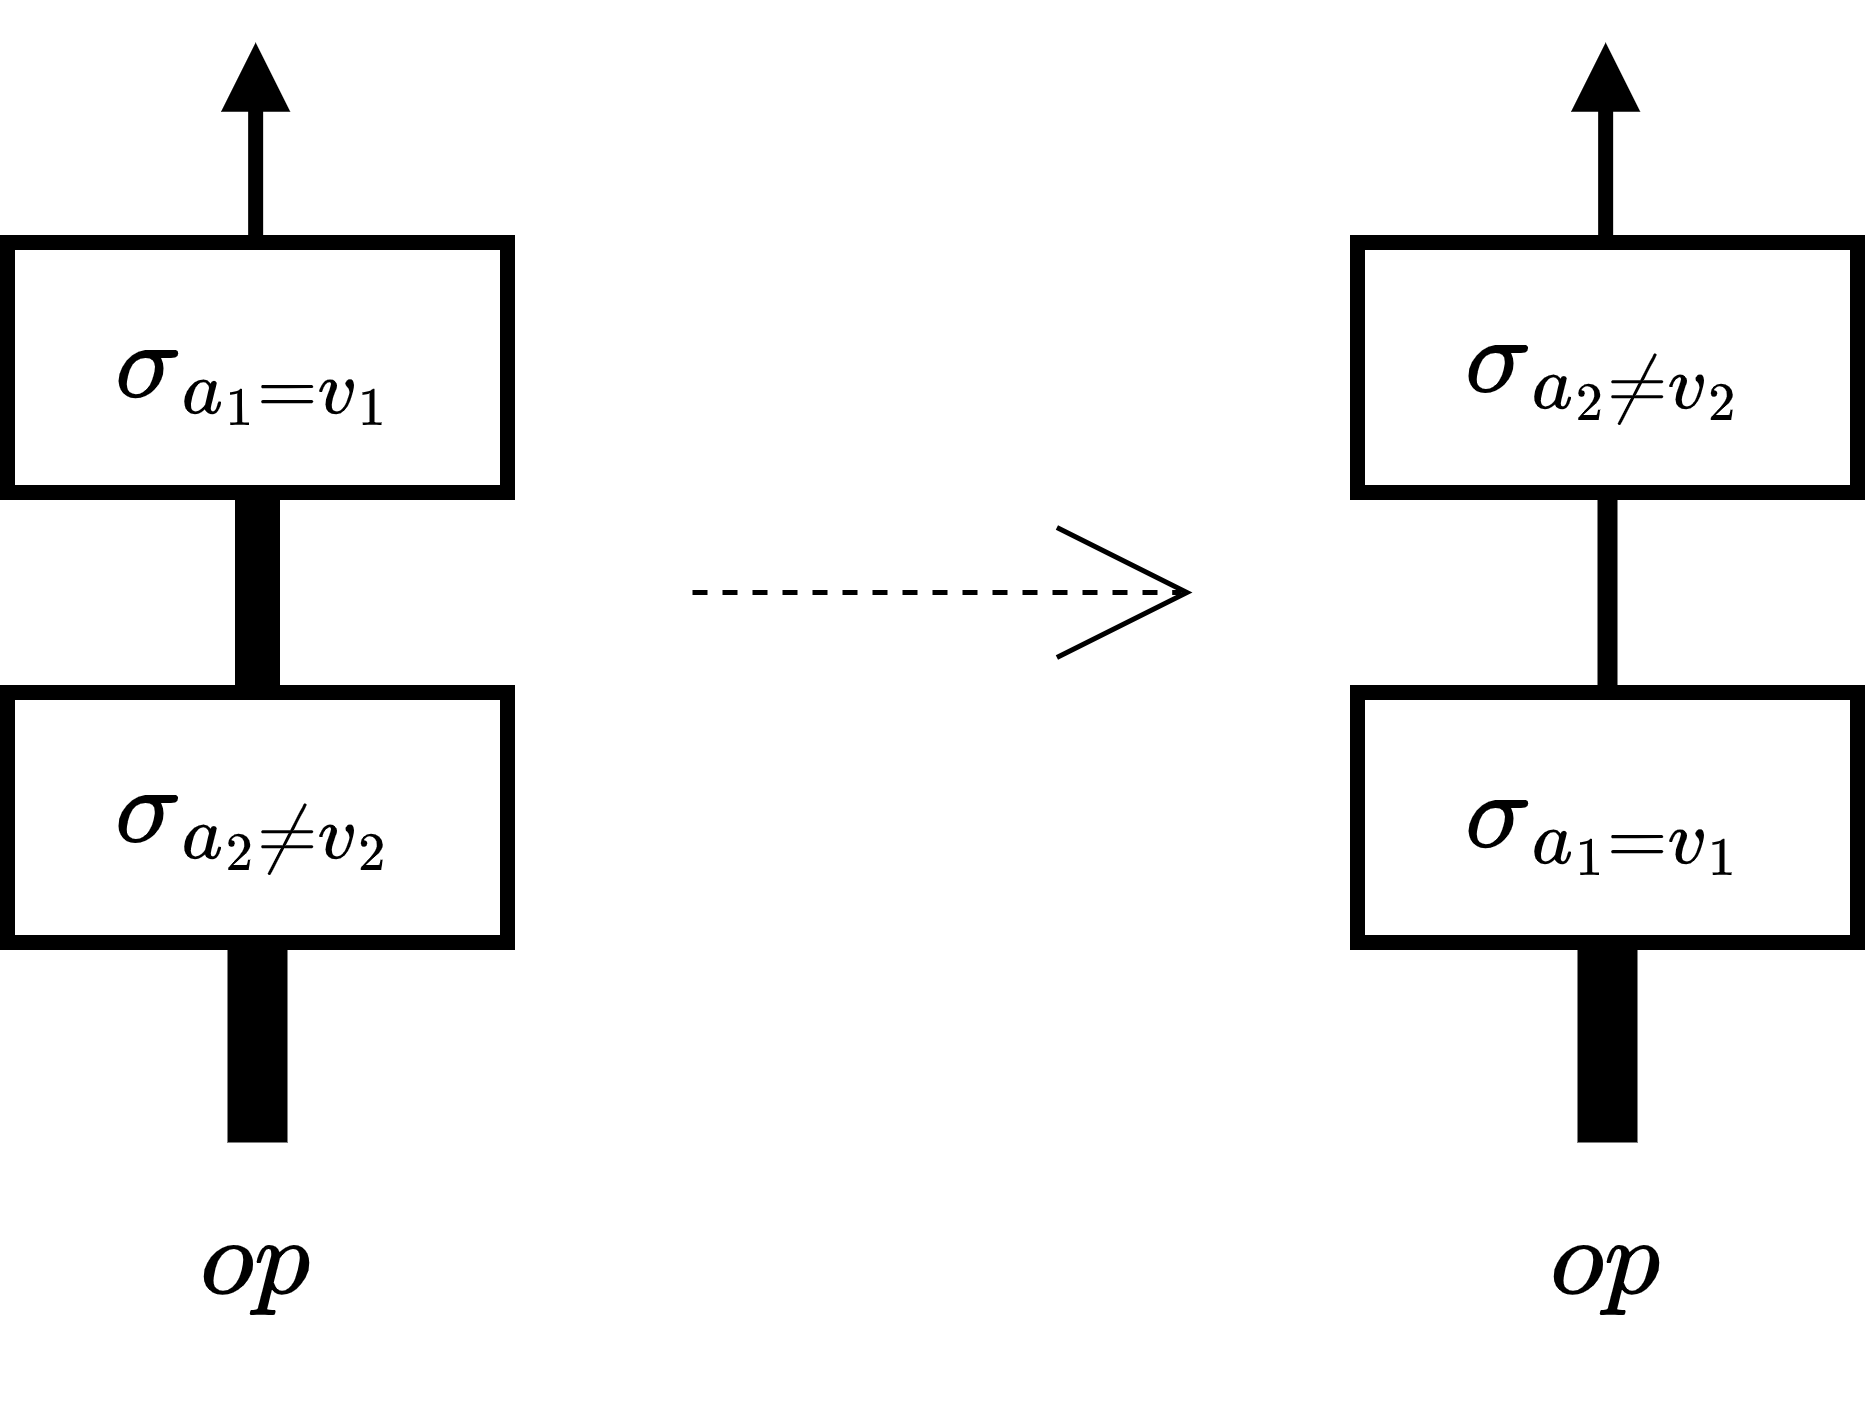
\includegraphics[width=.4\textwidth]{optimisation/images/selection_reordering.drawio.png}
\end{center}
Reordering selections to reduce cardinality at the earliest possible operator.
\begin{itemize}
    \item We infer which selection has the lowest selectivity using a heuristic
    \item A common heuristic for comparison operators: \mintinline{sql}{==} $ < $ ( \mintinline{sql}{<} and \mintinline{sql}{>} ) $ < $ ( \mintinline{sql}{<=} and \mintinline{sql}{>=} ) $ < $ \mintinline{sql}{<>}.
\end{itemize}
\begin{minted}{sql}
SELECT * FROM ( SELECT * FROM op WHERE a2 <> v2 ) WHERE a1 == v1; 
\end{minted}
\dots is optimised to \dots
\begin{minted}{sql}
SELECT * FROM ( SELECT * FROM op WHERE a1 == v1 ) WHERE a2 <> v2;
\end{minted}
\begin{minted}{haskell}
logicalRuleBased 
  (Select (Select op p1) p2) | p2 `predicateLess` p1 -- (with EQ < NEQ) 
  = Just (Select (Select op p2) p1)
\end{minted}

\subsubsection{Implication}
\begin{center}
    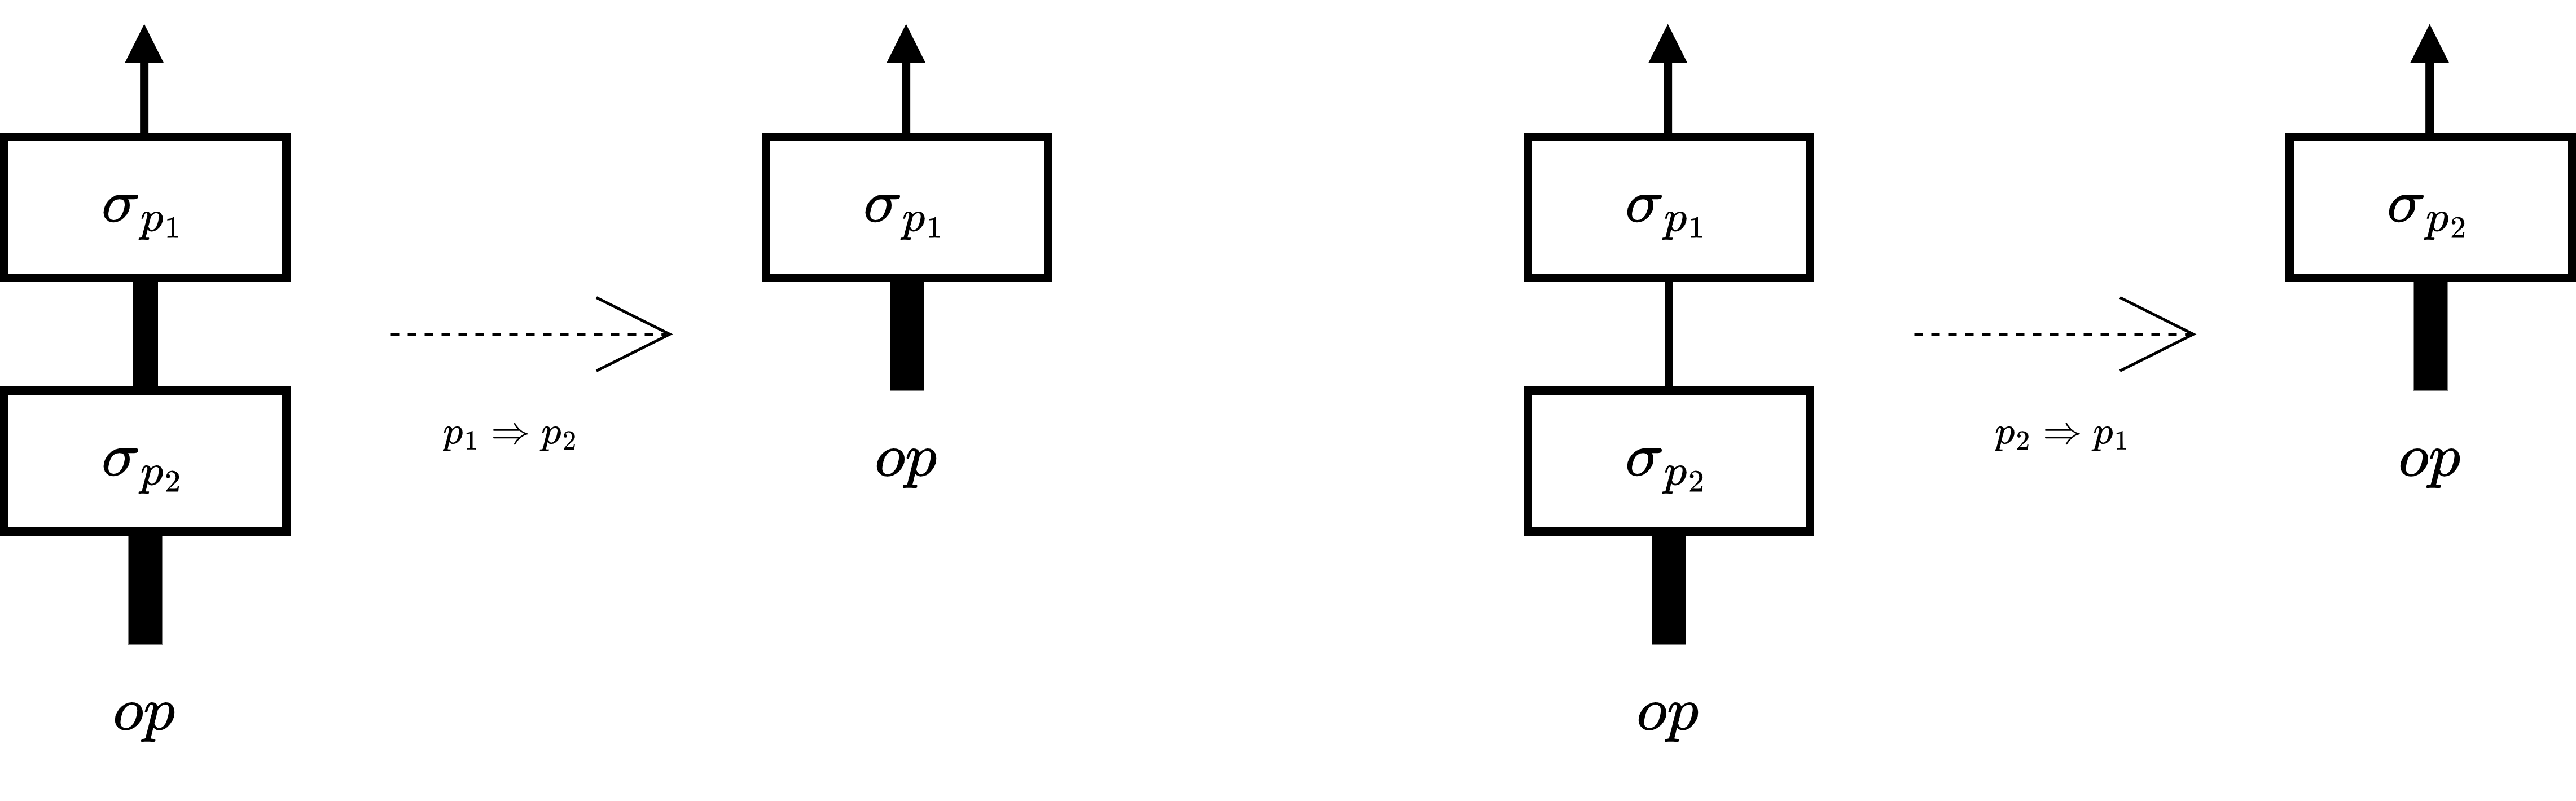
\includegraphics[width=.9\textwidth]{optimisation/images/implies_elimination.drawio.png}
\end{center}
Given one selection implies the other, we can eliminate another.
\begin{minted}{sql}
SELECT * FROM (SELECT * FROM op WHERE a1 == v1) WHERE a1 == v1 AND a2 == v2 
\end{minted}
\dots is optimised to \dots
\begin{minted}{sql}
SELECT * FROM op WHERE a1 == v1 AND a2 == v2 
\end{minted}
\begin{minted}{haskell}
logicalRuleBased
  (Select (Select op p1) p2) 
   | p1 `predicateImplies` p2 = Just (Select op p1)
   | p2 `predicateImplies` p1 = Just (Select op p2)  
\end{minted}

More sophisticated rules for simplifying, combining and eliminating selections are possible.

\subsection{Cost Based Logical Optimisation}
A cost metric is defined to determine which optimised plans are \textit{better/worse}.
\begin{minted}{haskell}
-- Types for query optimisation
type Selectivity = Double
type Cost        = Double

-- a function to determine the selectivity of a predicate
selectivity :: Predicate -> Cost

-- a heuristic for cost, using an estimate for the number of tuples output by an operator
sizeCost :: Operator -> Cost
sizeCost op = case op of
  Scan        t         -> fromIntegral (tableSize t)
  Select      op   p    -> selectivity p * sizeCost op
  Project     op   _    -> sizeCost op
  Product     opL opR   -> sizeCost opL * sizeCost opR
  Join        opL opR p -> selectivity p * sizeCost opL * sizeCost opR
  Difference  opL opR   -> max (sizeCost opL) (sizeCost opR)
  Union       opL opR   -> sizeCost opL + sizeCost opR
  Aggregation _   af    -> aggGroups af
  TopN        op  _  n  -> min (sizeCost op) n
\end{minted}
\mintinline{haskell}{Selectivity} needs to get an estimate. We will consider the basic case of an equality selection $\sigma_{a = v}$ where the possible values of $v$ are for attribute $a$ are know.
\subsubsection{Uniform Distribution}
If we assume all values are equally likely:
\[selectivity(a = v) \triangleq \cfrac{1}{\text{number of distinct values}}\]


\subsubsection{Histograms}
Store the frequency of values in a table.
\begin{center}
    \begin{minipage}{.49\textwidth}
        \begin{center}
            \begin{tabular}{l c c c c c}
                \multicolumn{6}{c}{$\underline{histogram_a}$}              \\
                \textbf{values}    & $v_1$ & $v_2$ & $v_3$ & \dots & $v_n$ \\
                \textbf{frequency} & $c_1$ & $c_2$ & $c_3$ & \dots & $c_n$ \\
            \end{tabular}
        \end{center}
    \end{minipage} \hfill \begin{minipage}{.49\textwidth}
        \[selectivity(a = v) \triangleq P(a = v) \equiv \cfrac{histogram_a.v}{histogram_a.total} \]
    \end{minipage}
\end{center}
\begin{itemize}
    \item Must retain and update a histogram for each attribute, with a count for each unique value.
    \item Histograms can be binned (like bitmap indices) when the number of unique values is large.
\end{itemize}
when evaluating multiple equalities, we assume \textit{attribute independence}, and hence:
\[selectivity(a_1 = v_1  \dots \land a_n = v_n) \equiv P(a_1 = v_1) \times \dots \times P(a_n = v_n) = \cfrac{histogram_{a_1}.v_1}{histogram_{a_1}.total} \times \dots \times \cfrac{histogram_{a_n}.v_n}{histogram_{a_n}.total}\]

\begin{sidenotebox}{Binned Histograms}
    SparkSQL's catalyst optimiser uses binned histograms as implemented \href{https://github.com/apache/spark/blob/master/sql/catalyst/src/main/scala/org/apache/spark/sql/catalyst/plans/logical/Statistics.scala}{here}
\end{sidenotebox}

\subsubsection{Multidimensional Histograms}
Often attribute values are correlated (e.g largest orders tend to be urgent).
\begin{center}
    \begin{tabular}{l l c c c c c}
        \multicolumn{7}{c}{$\underline{histogram_{(a_1, a_2)}}$}                                                                                             \\
                                         &               & \multicolumn{5}{c}{attribute $a_1$}                                                               \\
                                         &               & ${v_{a_1}}_1$                       & ${v_{a_1}}_2$ & ${v_{a_1}}_3$ & \dots       & ${v_{a_1}}_n$ \\
        \multirow{5}{*}{attribute $a_2$} & ${v_{a_2}}_1$ & $c_{(1,1)}$                         & $c_{(2,1)}$   & $c_{(3,1)}$   & $c_{(4,1)}$ & $c_{(5,1)}$   \\
                                         & ${v_{a_2}}_2$ & $c_{(1,2)}$                         & $c_{(2,2)}$   & $c_{(3,2)}$   & $c_{(4,2)}$ & $c_{(5,2)}$   \\
                                         & ${v_{a_2}}_3$ & $c_{(1,3)}$                         & $c_{(2,3)}$   & $c_{(3,3)}$   & $c_{(4,3)}$ & $c_{(5,3)}$   \\
                                         & \vdots        & $c_{(1,4)}$                         & $c_{(2,4)}$   & $c_{(3,4)}$   & $c_{(4,4)}$ & $c_{(5,4)}$   \\
                                         & ${v_{a_2}}_n$ & $c_{(1,5)}$                         & $c_{(2,5)}$   & $c_{(3,5)}$   & $c_{(4,5)}$ & $c_{(5,5)}$   \\
    \end{tabular}
\end{center}

\begin{itemize}
    \item Store multiple histograms to show frequencies of attribute values, given other attribute's value.
    \item Number of histograms grows combinatorially with number of tables.
    \item Reducing the number of histograms, but still producing good selectivity estimates is an open area of research.
\end{itemize}
\[selectivity(a_1 = v_1 \land a_2 = v_2) = P(a_1 = v_1 | a_2 = v_2) \times P(a_2 = v_2) = \cfrac{histogram_{(a_1, a_2)}.(v_1, v_2)}{histogram_{(a_1, a_2)}.total} \]

\section{Physical Optimisation}
\begin{definitionbox}{Physical Plan}
    A plan containing implementation specific information, and describing how the query should be physically executed.
    \begin{itemize}
        \item Operator implementations (e.g which join: sort-merge, hash, nested loop, index based join etc)
        \item Costs of different implementations (e.g hash join vs nested-loop $\to$ time versus memory)
        \item Available indices \& data structure choices (e.g type of hashmap, hash function)
    \end{itemize}
    Physical plan optimisation focuses on optimising the plan for the specific system the query is executed on.
\end{definitionbox}

The cost metric different types of cost (e.g time versus memory)
\begin{itemize}
    \item Produced tuples
    \item Page faults
    \item Intermediate buffer sizes
    \item (Volcano Processing) function calls
    \item Storage access \& availability
\end{itemize}
We can then decide if a rule is universally beneficial (for \textit{rule-based}), or determine which possible plan is lowest cost (\textit{cost-based})

\subsection{Rule Based Physical Optimisation}
Much like \textit{logical rule-based optimisation}, (almost) universally beneficial (given the decided cost metric) rules to improve performance.
\begin{center}
    \begin{tabular}{l p{.8\textwidth}}
        \textbf{Data structures} & Always use hash map with rehashing for probe if expected collisions are high.                                                \\
        \textbf{Parallelism}     & always use parallel sort for \mintinline{sql}{ORDER BY}, always partition hash joins                                         \\
        \textbf{Using Indices}   & If foreign key index exists, always use for foreign key join, if getting range always use available bitmap or B+ tree index. \\
        \textbf{Cache}           & Always use cache-conscious partitioning to improve locality.                                                                 \\
    \end{tabular}
\end{center}

\subsection{Cost Based Physical Optimisation}
Much like \textit{logical cost-based optimisation} but on a physical plan (using implementation specific details).
\begin{center}
    \begin{tabular}{l p{.8\textwidth}}
        \textbf{Data}      & Consider cardinalities \& how this affect operator choice (e.g choose sort-merge join over hash if the required hashtable is too large for the buffer pool). \\
        \textbf{Hardware}  & Function call overhead (for this architecture), buffer pool size, access latencies, available parallelism (hardware threads).                                \\
        \textbf{Algorithm} & Must consider how algorithms expected costs change with parameters (e.g cardinality)                                                                         \\
    \end{tabular}
\end{center}
This is the current state of the art in optimisation.

\section{SparkSQL}
\begin{sidenotebox}{SparkSQL Logical Optimiser}
    You can find the source for SparkSQL's catalyst optimiser's logical optimisations \href{https://github.com/apache/spark/blob/master/sql/catalyst/src/main/scala/org/apache/spark/sql/catalyst/optimizer/Optimizer.scala}{here on github}.
\end{sidenotebox}
\begin{center}
    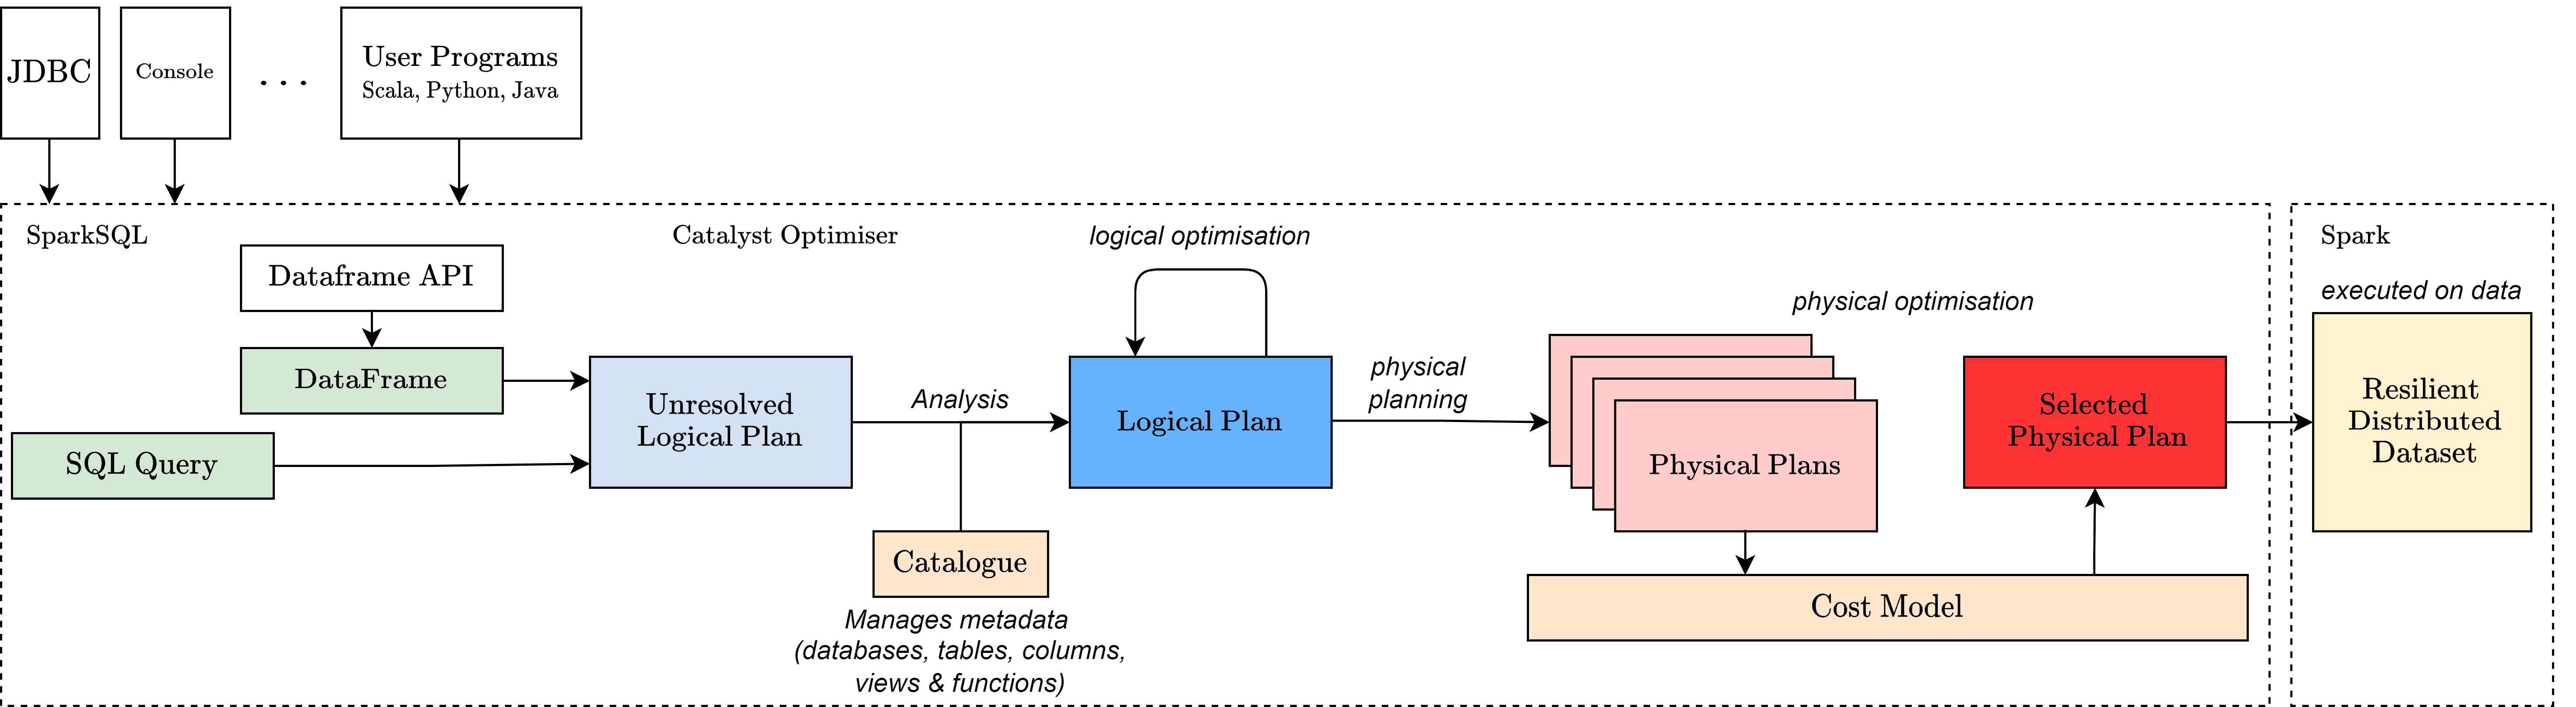
\includegraphics[width=\textwidth]{optimisation/images/catalyst.drawio.png}
\end{center}
\begin{itemize}
    \item \textit{Rule-based logical optimiser} and \textit{cost-based physical optimiser}
    \item Rather than reapplying the physical plan optimiser repeatedly on one plan, multiple possible candidate plans are produced and evaluated (negates local optima problem at the cost of generating many physical plans).
\end{itemize}
\noindent
Logical rules are expressed as extensions of a \mintinline{scala}{Rule[LogicalPlan]} interface. For example expression simplification and constant folding can be found in the \href{https://github.com/apache/spark/blob/master/sql/catalyst/src/main/scala/org/apache/spark/sql/catalyst/optimizer/expressions.scala}{expression optimiser}.
\begin{minted}{scala}
/**
* Simplifies boolean expressions:
* 1. Simplifies expressions whose answer can be determined without evaluating both sides.
* 2. Eliminates / extracts common factors.
* 3. Merge same expressions
* 4. Removes `Not` operator.
*/
object BooleanSimplification extends Rule[LogicalPlan] with PredicateHelper {
  def apply(plan: LogicalPlan): LogicalPlan = plan.transformWithPruning(
    _.containsAnyPattern(AND, OR, NOT), ruleId) {
    case q: LogicalPlan => q.transformExpressionsUpWithPruning(
      _.containsAnyPattern(AND, OR, NOT), ruleId) {
        case TrueLiteral And e => e
        case e And TrueLiteral => e
        case FalseLiteral Or e => e
        case e Or FalseLiteral => e
        // ...
      }
      // ...
    }
}
\end{minted}
